\documentclass{book}
\usepackage[a4paper, margin=1in]{geometry}
\usepackage{amsmath}
\usepackage{amsthm}

% Define the 'definition' environment
\newtheorem{definition}{Definition}
\usepackage{amssymb}
\usepackage{tcolorbox}
\usepackage{amsthm}
\usepackage{graphicx}
\usepackage[hidelinks]{hyperref}
\usepackage{cleveref}
\usepackage{float}
\usepackage{subcaption}
\usepackage{tikz}
\usepackage{tocloft}
\usepackage{algorithm}
\usepackage{algpseudocode}
\usepackage[english]{babel}
\usepackage{makecell}
\setlength{\parindent}{0pt}
\setlength{\parskip}{6pt}


\title{Distributed Systems}
\author{Alessandro Dori}
\date{\today}

\begin{document}

\begin{titlepage}
    \centering
        \vspace*{1in}
        
        
\includegraphics[width=0.4\textwidth]{Immagini/logo-sapienza.png}\par\vspace{1cm}
        
        {\scshape\LARGE Sapienza University of Rome \par}
        \vspace{1.5cm}

         {\scshape\Large Distributed Systems Notes\par}
        \vspace{1.5cm}
        
        {\Large\itshape Alessandro Dori\par}
        
        \vspace{3cm}
        
        Instructor:\par
        {\large Prof. Giuseppe Antonio Di Luna\par}
        
        \vfill
        
        {\large Academic Year 2025/2026\par}
    
\end{titlepage}

\maketitle
\tableofcontents
\setcounter{tocdepth}{2} % Adjust the depth of the table of contents to avoid bookmark level issues
\newpage

\chapter{Introduction}
Distributed computing addresses algorithms for a set of processes that seek to achieve some form of cooperation.
Some of the processes of a distributed system might stop operating, for instance, by crashing or beign disconnected, while others might stay alive and keep operating.
This very notion of \textit{partial failures} is a characteristic of a distributed system.

\begin{definition}
    A distributed system is a set of \textbf{spatially separate entities}, each of these with a \textbf{certain computational power} that are able to communicate and to coordinate among themselves for reaching a common goal.\\
\end{definition}

\begin{tcolorbox}[colback=blue!5!white,colframe=blue!75!black,title=Leslie Lamport on Distributed Systems]
    A distributed system is one in which the \textbf{failure} of a computer you didn't even know existed can render your own computer unusable.
    \begin{flushright}
        \textit{--- Leslie Lamport}
    \end{flushright}
\end{tcolorbox}

When a subset of the processes have failed, or become disconnected, the challenge is usually for the processes that are still operating, or connected to the majority of the processes, to synchronize their activity in a consistent way.
\newline
Due to the asynchrony of the processes, he possibility of failures in the communication infrastructure, and perhaps even malicious actions by faulty processes, it may be impossible to accurately detect process failures; in particular, there is often no way to distinguish a process failure from a network failure.
\newline
Even worse, a process that is under the control of a malicious adversary may misbehave deliberately, in order to disturb the communication among the remaining processes.
The challenge in distributed computing is precisely to devise algorithms that provide the processes that remain operating with enough consistent information so that they can cooperate correctly and solve common tasks.

\begin{itemize}
    \item \textbf{Examples of Distributed Systems:}
    \begin{itemize}
        \item The Internet
        \item The World Wide Web
        \item Peer-to-peer systems (e.g., BitTorrent)
        \item Cloud computing platforms (e.g., AWS, Google Cloud)
        \item Distributed databases (e.g., Cassandra, MongoDB)
        \item Blockchain networks (e.g., Bitcoin, Ethereum)
    \end{itemize}
    \item \textbf{Common points across definitions}
        \begin{itemize}
            \item \textbf{Set of entities}: computers, machines, software;
            \item \textbf{Distributed}: spatially separated, independent;
            \item \textbf{Common Goal}: communication, coordination, resource sharing;
        \end{itemize}
\end{itemize}


\section{Distributed Programming Abstractions}
By capturing properties that are common to a large significant range of systems, abstractions help distinguish the fundamental from the accessory, and prevent system designers and engineers from reinventing the same solutions for slight variants of the very same problems.

The processes of a distributed program abstract the active entities that perform computations. 
A process may represent a computer, a processor within a computer, or simply a specific thread of execution within a processor. 
In the context of network security, a process may also represent a trust domain, a principal, or one administrative unit. 
To cooperate on some common task, the processes may typically need to exchange messages using some communication network. 
Links abstract the physical and logical network that supports communication among processes. 
It is possible to represent multiple realizations of a distributed system by capturing different properties of processes and links, for instance, by describing how these elements may operate or fail under different environmental conditions.

The cooperation among processes can sometimes be modeled as a distributed agreement problem. 
For instance, the processes may need to agree on whether a certain event did (or did not) take place, to agree on a common sequence of actions to be performed (from a number of initial alternatives), or to agree on the order by which a set of inputs need to be processed. 
It is desirable to establish more sophisticated forms of agreement from solutions to simpler agreement problems, in an incremental manner.

\subsection{Inherent Distribution}
Applications that require sharing or dissemination of information among several participant processes are a fertile ground for the emergence of problems that required distributed programming abstractions.

\paragraph{Information Dissemination.}
In distributed applications with information dissemination requirements, processes may play one of the following roles:
information producers (\textit{publishers}), information consumers (\textit{subscribers}).
\newline
Publisher produce information in the form of notifications.
Subscribers register their interest in receiving cerain notifications.
\newline
Independently of the subscription method, it is very likely that several subscribers are interested in the same notifications, which the system should broadcast to them.
In this case, we are typically interested in having all subscribers of the same information receive the same set of messages.
Otherwise the system will provide an unfair service, as some subscribers could have access to a lot more information than other subscribers.
\newline
Unless this reliability property is given for free by the underlying infrastructure, the sender and the subscribers must coordinate to agree on which messages should be delivered.
For instance, with the dissemination of an audio stream, processes are typically interested in receiving most of the information but are able to tolerate a bounded amount of message loss.
The corresponding abstraction is typically called a \textbf{best-effort broadcast}.
\newline
The dissemination of some stock exchange information may require a more reliable form of broadcast, called \textbf{reliable broadcast}, which guarantees that if a correct process receives a message, then all correct processes receive it.

\paragraph{Process Control.}
Process control applications are those where several software processes have to control the executionn of a physical acrivity.
\newline
Typically, every process is connected to some sensor.
The processes might, for instance, need to exchange the values output by their assigned sensors and output some common value, despite the fact that, due to the inaccuracy of failure of their local sensors, they may have observed slightly different input values.
This cooperation should be achieved despite some sensors (or associated control processes) having crashed or not observed anything.
This type of cooperation can be simplified if all processes agree on the same set of inputs for the control algorithm, a requirement captured by the \textit{consensus} abstraction.

\newpage
\paragraph{Cooperative Work.}
Users located on different nodes of a network may cooperate
in building a common software or document, or simply in setting up a distributed
dialogue, say, for an online chat or a virtual conference. A shared working space
abstraction is very useful here to enable effective cooperation. Such a distributed
shared memory abstraction is typically accessed through read and write operations
by the users to store and exchange information. In its simplest form, a shared working space can be viewed as one virtual unstructured storage object. 
In more complex incarnations, shared working spaces may add a structure to create separate locations for its users to write, and range all the way from Wikis to complex multiuser
distributed file systems. To maintain a consistent view of the shared space, the processes need to agree on the relative order among write and read operations on the
space.

\paragraph{Distributed Databases.}
Databases constitute another class of applications where
agreement abstractions can be helpful to ensure that all transaction managers obtain
a consistent view of the running transactions and can make consistent decisions on
how these transactions are serialized.
\newline
Additionally, such abstractions can be used to coordinate the transaction managers when deciding about the outcome of the transactions. That is, the database servers, on which a given distributed transaction has executed, need to coordi-
nate their activities and decide whether to commit or abort the transaction. They
might decide to abort the transaction if any database server detected a violation of
the database integrity, a concurrency control inconsistency, a disk error, or simply
the crash of some other database server. As we pointed out, the distributed programming abstraction of atomic commit (or commitment) provides such distributed
cooperation.

\paragraph{Distributed Storage.}
A large-capacity storage system distributes data over many
storage nodes, each one providing a small portion of the overall storage space.
Accessing stored data usually involves contacting multiple nodes because even a
single data item may be spread over multiple nodes. A data item may undergo
complex transformations with error-detection codes or error-correction codes that
access multiple nodes, to protect the storage system against the loss or corruption of
some nodes. Such systems distribute data not only because of the limited capacity
of each node but also for increasing the fault-tolerance of the overall system and for
reducing the load on every individual node.
Conceptually, the storage system provides a shared memory abstraction that is
accessed through read and write operations, like the shared working space mentioned before. But since it uses distribution also for the purpose of enhancing the
overall resilience, it combines aspects of inherently distributed systems with aspects
of artificially distributed systems, which are discussed next.


\section{Software Components}
\subsection{Composition Model}
One of the biggest difficulties we had to face when thinking about describing distributed algorithms was to find an adequate way to represent these algorithms.
\newline
Therefore, we have opted to use pseudo code to describe our algorithms.
The pseudo code reflects a reactive computing model where components of the same process communicate by exchanging events: an algorithm is described as a set of event handlers.
These react to incoming events and possibly trigger new events.

We shall describe algorithms using an asynchronous event-based composition model.
Every process hosts a set of software components, called modules in our context.
Each component is identified by a name, and characterized by a set of properties.

Distributed programming abstractions are typically made of a collection of components, at least one for every process, that are intended to satisfy some common properties.

\paragraph{Software Stacks.}
Components can be composed to build software stacks.
At each process, a component represents a specific layer in the stack.
The layers of the distributed programming abstractions we will consider are typically in the middle.
Components within the same stack communicate through the exchange of events.
A given abstraction is typically materialized by a set of components, each running at a process.

According to this model, each component is constructed as a state-machine whose transitions are triggered by the reception of events.
Events may carry information such as a data message, or group membership information, in one or more attributes.
Events are denoted by $\langle \text{\textit{EventType}} \mid \text{\textit{Attributes, }} \ldots \rangle$. 

Often an event with the same name is used by more than one component.
For events defined for component \textit{co}, we, therefore, usually write:

$
\qquad \langle \text{\textit{co,EventType}} \mid \text{\textit{Attributes, }} \ldots \rangle
$

Each event is processed through a dedicated \textit{handler} by the process.
A handler is formulated in terms of a sequence of instructions introduced by \textit{upon event}, which describes the event, followed by pseudocode with instructions to be executed.
The processing of an event may result in new events being created and triggering the same or different components.
Every event triggered by a component of the same process is eventually processed, if the process is correct.

The pseudo code of a sample component $co_1$ that consists of two event handlers looks like this:

\begin{center}
    \begin{algorithmic}
    \State \textbf{upon event} $\langle co_1, Event_1 \mid att_{1}^1, att_{1}^2, \ldots \rangle$ \textbf{do}
    \State \quad do something;
    \State \quad \textbf{trigger} $\langle co_2, Event_2 \mid att_{2}^1, att_{2}^2, \ldots \rangle$;
    \Statex
    \State \textbf{upon event} $\langle co_1, Event_3 \mid att_{3}^1, att_{3}^2, \ldots \rangle$ \textbf{do}
    \State \quad do something else;
    \State \quad \textbf{trigger} $\langle co_2, Event_4 \mid att_{4}^1, att_{4}^2, \ldots \rangle$;
    \end{algorithmic}
\end{center}

For writing complex algorithms, we sometimes use handlers that are triggered when some condition in the implementation becomes true, but do not respond to an external event originating from another module.
The condition for an internal event is usually defined on local variables maintained by the algorithm. 
Such a handler consists of an upon statement followed by a condition; in a sample component \textit{co}, it might look like this:

\begin{center}
    \begin{algorithmic}
    \State \textbf{upon} condition \textbf{do}
    \State \quad do something;
    \end{algorithmic}
\end{center}

An upon event statement triggered by an event from another module can also be qualified with a condition on local variables.
This handler executes its instructions only when the external event has been triggered and the condition holds.
Such a conditional event handler of a component \textit{co} has the following form:

\begin{center}
    \begin{algorithmic}
    \State \textbf{upon event} $\langle co, Event \mid att_{1}^1, att_{1}^2, \ldots \rangle$ \textbf{auch that} condition \textbf{do}
    \State \quad do something;
    \end{algorithmic}
\end{center}

An algorithm that uses conditional event handlers relies on the run-time system to
buffer external events until the condition on internal variables becomes satisfied.
We use this convention because it simplifies the presentation of many algorithms, but the approach should not be taken as a recipe for actually implementing a practical system: such a run-time system might need to maintain unbounded buffers.
But, it is not difficult to avoid conditional event handlers in an implementation.
Every conditional event handler can be transformed into a combination of a (pure) event handler and two handlers for internal events in three steps: 
(1) introduce a local variable for storing the external event when it occurs and install an event handler triggered by the external event without any condition; 
(2) introduce a local variable for storing that the condition on the internal variables has become true; and 
(3) add a local event handler that responds to the internal event denoting that the external event has occurred and the internal condition has been satisfied.


\subsection{Programming Interface}
The APIs of our components include two types of events, \textit{requests} and \textit{indications};
their detailed semantics depend on the component at which they occur:
\begin{itemize}
    \item A \textbf{request} event is triggered by a component to request a service from another component, typically at the same process. 
    The request event is usually triggered by an event handler of the requesting component.
    \item An \textbf{indication} event is triggered by a component to indicate that some event has occurred, typically at the same process. 
    The indication event is usually triggered by an event handler of the indicating component.
\end{itemize}

\begin{center}
    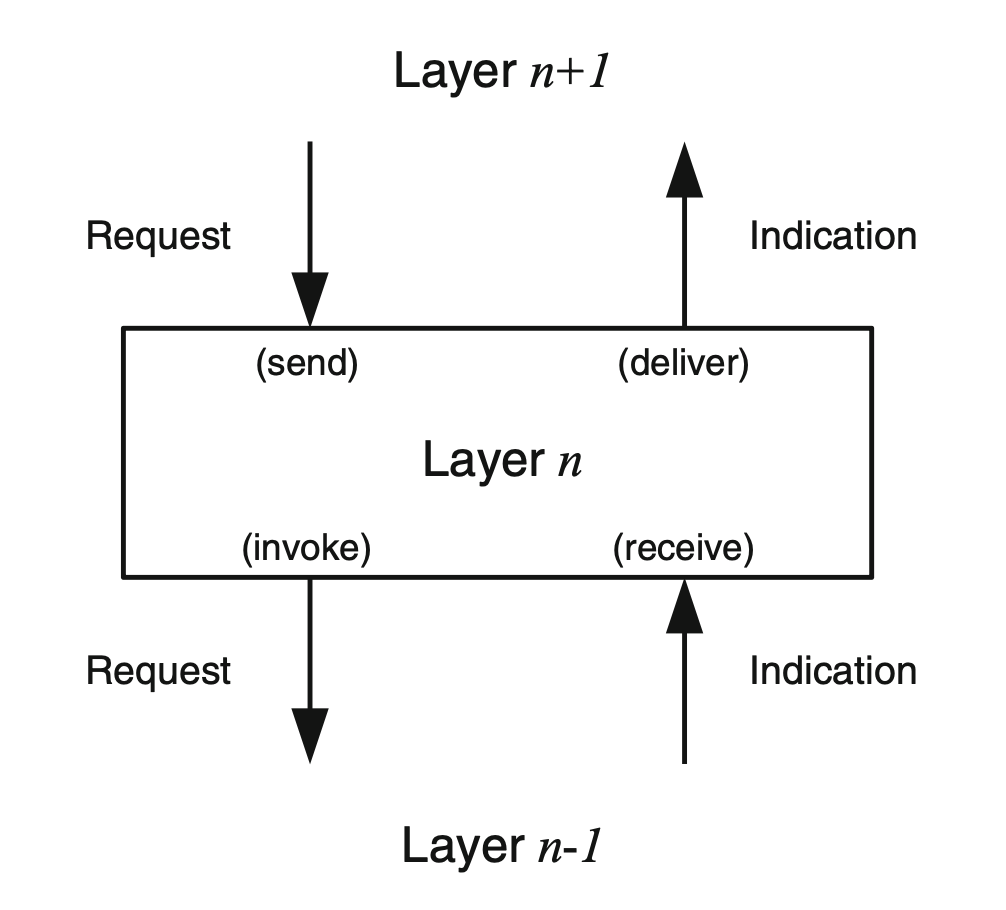
\includegraphics[width=0.4\textwidth]{Immagini/6.png}
\end{center}

Requests and indications do not always carry payload data; they may also indicate
conditions for synchronizing two layers with each other.
For example, the broadcast abstraction may confirm that its service has been concluded reliably by triggering a specialized indication event for the layer above. 
In this way, a broadcast implementation can require that the application layer waits until a broadcast request is confirmed before triggering the next broadcast request.
An analogous mechanism can be used to synchronize the delivery of broadcast messages to the application layer above.
When the application layer takes a long time to process a message, for example, the application may trigger a specialized request event for the broadcast abstraction to signal that the processing has completed and the application is now ready for the next broadcast message to be delivered.


\chapter{Basic Abstractions}
\section{Model}
\subsection{System and Processes}

\begin{definition}
    A system is a set of \textbf{processes} that communicate and coordinate to achieve a common goal.
\end{definition}
\begin{itemize}
    \item We have $n$ processes (where $n$ is fixed and we know the identities) in $\Pi = \{p_0, p_1, \ldots, p_{n-1}\}$ with \textbf{distinct} identities.
    \item Processes communicate using a communication graph $G = (\Pi, E)$ where $E \subseteq \Pi \times \Pi$ (usually, $G$ is a complete graph).
    \item The communication happens by exchanging messages on communication links (edges of $G$), and messages are uniquely identified, say, by their original sender process using a sequence number or a local clock, together with the process identifier.
\end{itemize}
\begin{center}
    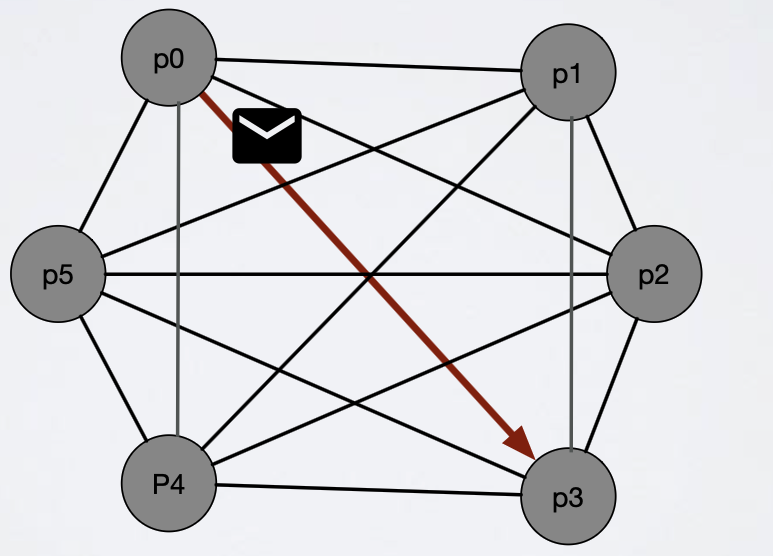
\includegraphics[width=0.3\textwidth]{Immagini/1.png}
\end{center}

A process is a (possibly infinite) State Machine (I/O Automation).
\begin{center}
    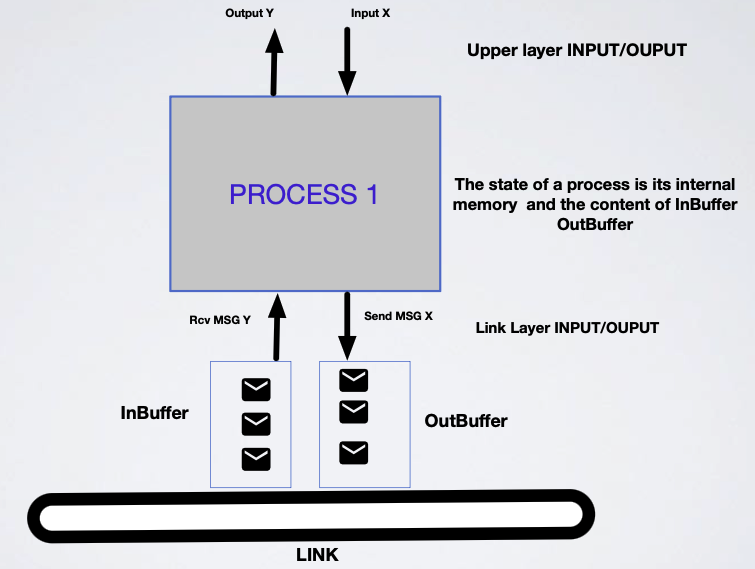
\includegraphics[width=0.3\textwidth]{Immagini/2.png}
\end{center}
\begin{itemize}
    \item Internal states - set Q
    \item Initial state - $Q_i \subset Q$
    \item Messages - set of all possible messages M in the form 
    $$\langle \text{sender}, \text{receiver}, \text{payload} \rangle$$
    \item $\text{InBuf}_j$ - multiset of delivered messages
    \item $\text{OutBuf}_j$ - multiset of "inflight" messages (messages sent but not delivered).
\end{itemize}
$$
\text{P}_j\left(q \in Q \cup Q_{in}, InBuf_j\right) = 
\left(q^{'} \in Q, Send\_msg \subset M\right) 
$$
$$
OutBuf_j = OutBuf_j \cup Send\_msg
$$
$$
InBuf_j = \emptyset
$$


\subsection{Asynchronous Executions}


\subsubsection{Execution}
There is an \textbf{adversary} that schedule a set of events (scheduler):
\begin{itemize}
    \item Delivery of a msg - $Del(m, i, j)$: move message $m$ from $OutBuf_i$ to $InBuf_j$;
    \item Execution of a local step - $Exec(i)$: process $i$ executes one step of its state machine.
\end{itemize}

\begin{center}
    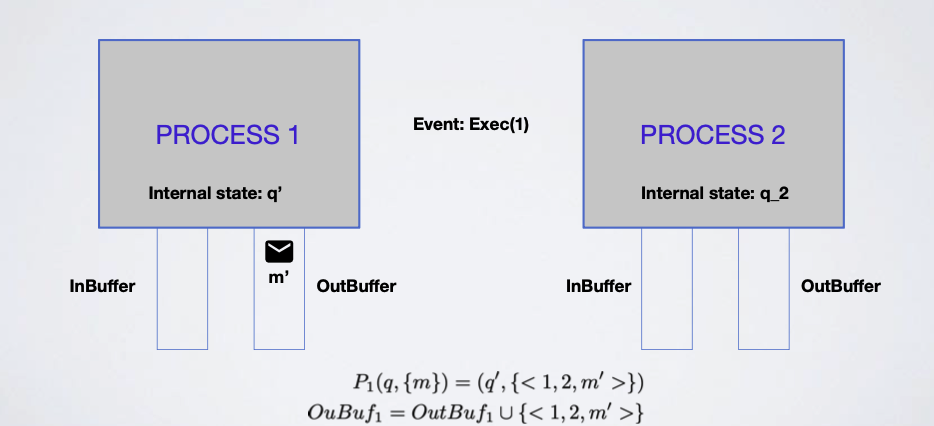
\includegraphics[width=0.4\textwidth]{Immagini/3.png}
    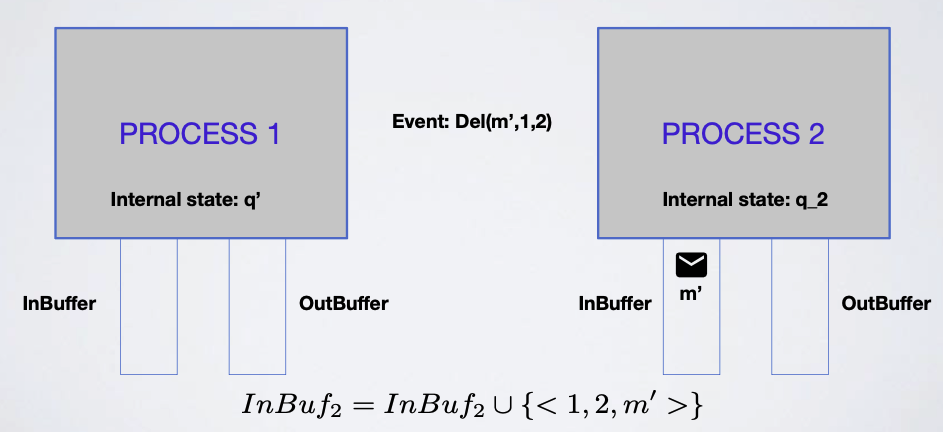
\includegraphics[width=0.4\textwidth]{Immagini/4.png}
\end{center}

A configuration $C_t$ is a vector of $n$ components. 
Component $j$ indicates the state of processes $j$ $\left(\text{that is } C_t[j] \left(q_i,InBuff_j,OutBuf_j\right)\right)$.

\begin{center}
    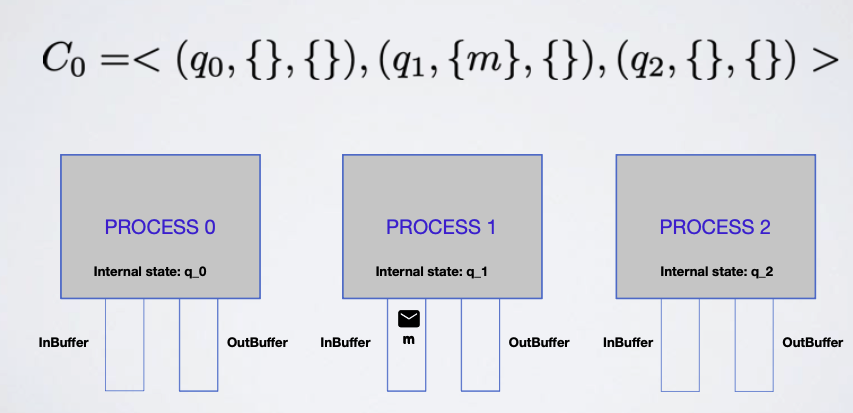
\includegraphics[width=0.4\textwidth]{Immagini/5.png}
\end{center}

It is convenient for presentation simplicity to assume the existence of a global clock, outside the control of the processes.
This clock provides a global and linear notion of time that regulates the execution of the algorithms. 
The steps of the processes are executed according to ticks of the global clock: one step per clock tick.

Unless specified otherwise, we will consider deterministic algorithms. 
That is, for every step performed by any given process, the local computation executed by the process, the local state after the computation, and the message sent by this process are uniquely determined by the message received by the process and its local state prior to executing the step.


\subsection{Safety and Liveness}
When we devise a distributed algorithm to implement a distributed programming abstraction, we seek to satisfy the properties of the abstraction in all possible executions of the algorithm, covering all possible sequences of steps executed by the processes according to the algorithm.
The scheduling of these steps remains outside the control of the processes and depends on the global scheduler.
The properties of the abstraction to be implemented needs to be satisfied for a large set of possible interleavings of these steps.
These properties usually fall into two classes: \textit{safety} and \textit{liveness}.

\paragraph{Safety.}
Basically, a safety property is a property of a distributed algorithm that can be violated at some time t and never be satisfied again after that time.
\newline
More precisely, a safety property is a property such that, whenever it is violated in some execution $E$ of an algorithm, there is a partial execution $E'$ of $E$ such that the property will be violated in any extension of $E'$.
This means that safety properties prevent a set of unwanted execution prefixes from occurring.

\paragraph{Liveness.}
They ensure that eventually something good happens. 
For instance, to define a meaningful notion of perfect links, we require that if a correct process sends a message to a correct destination process, then the destination process should eventually deliver the message.
To state that such a liveness property is violated in a given execution, we need to show that there is an infinite scheduling of the steps of the algorithm where the message is never delivered.
\newline
More precisely, a liveness property is a property of a distributed system execution such that, for any time $t$, there is some hope that the property can be satisfied at some time $t' \geq t$.

\paragraph{Combining them.}
The challenge is to guarantee both liveness and safety.
Consider, for instance, the traditional interprocess communication service of a reliable, ordered data stream: it ensures that messages exchanged between two processes are neither lost or nor duplicated, and are received in the order in which they were sent.
As we pointed out, requiring that messafes are not lost in a liveness property.
Requiring that messages are not duplicated and that they are received in the order in which they were sent are safety properties.

\begin{figure}[H]
    \centering
    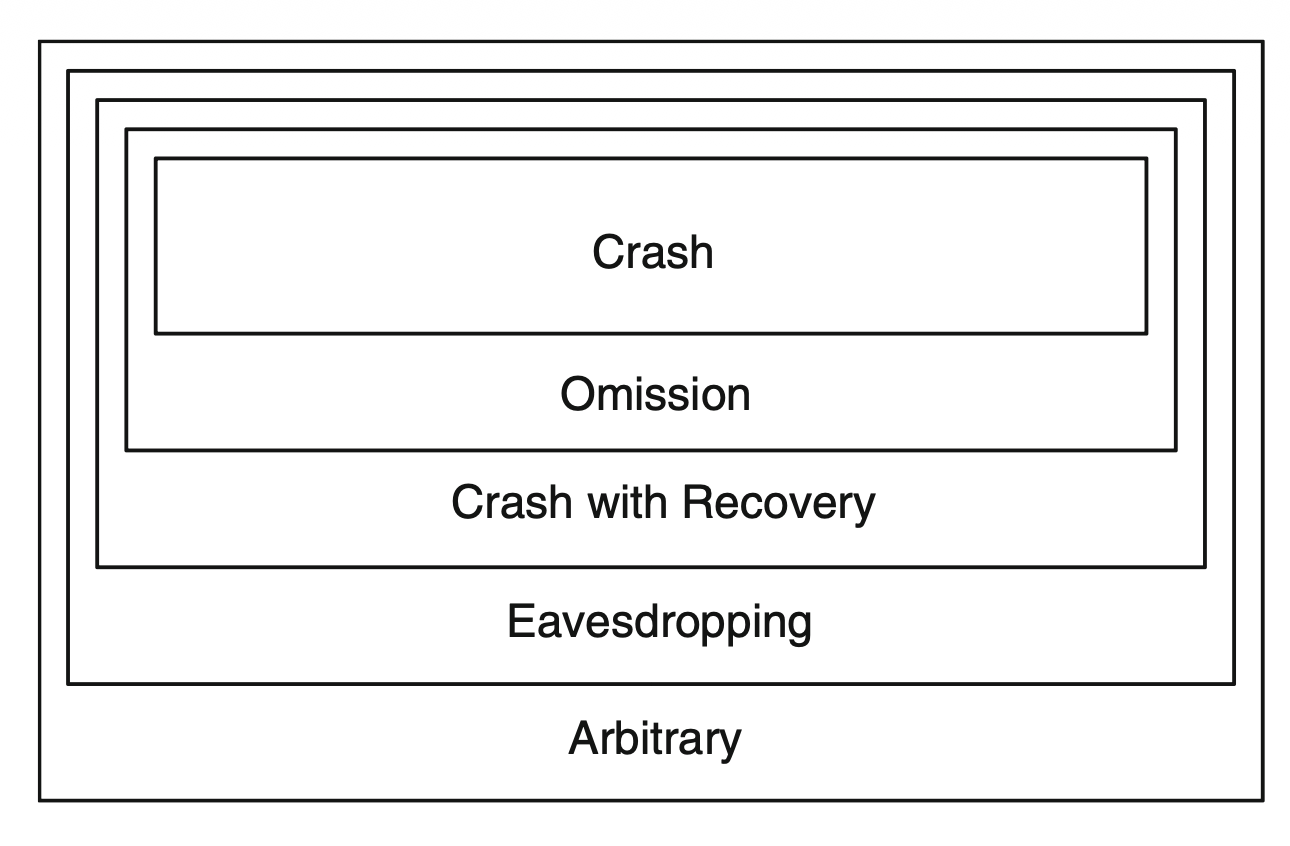
\includegraphics[width=0.4\textwidth]{Immagini/7.png}
    \caption{Types of process failures}
\end{figure}

\begin{tcolorbox}[colback=red!5!white,colframe=red!75!black,title=Failures]
All computer systems fail. It is a good design practice to build robust systems.

\begin{itemize}
    \item \textbf{Failure detection}: checksum detects a corrupted packet
    \item \textbf{Failure masking}: message retransmission, redundancy
    \item \textbf{Failure tolerance}: intrusion tolerance systems
    \item \textbf{Failure recovery}: backup and restore
\end{itemize}
\end{tcolorbox}


\section{Abstracting Processes}
\subsection{Process Failures}
A process executes the distributed algorithm assigned to it through the set of components implementing the algorithm within that process. A failure occurs whenever
the process does not behave according to the algorithm. Our unit of failure is the
process. When the process fails, all its components fail at the same time.
Process abstractions differ according to the nature of the faults that cause them
to fail. Possible failures range from a crash, where a process simply stops to execute
any steps, over an omission to take some steps, a crash with subsequent recovery,
to arbitrary and even adversarial behavior.

\subsection{Crashes}
The simplest way of failing for a process is when the process stops executing steps.
The process executes its algorithm correctly, including the exchange of messages with other processes, until some time $t$, after which it stops executing any local computation and does not send any message to other processes.
In other words, the process crashes at time $t$ and never recovers after that time.
We call this a crash fault, and talk about a crash-stop process abstraction.
With this abstraction, a process is said to be \textit{faulty} if it crashes at some time during the execution.
It is said to be correct if it never crashes and executes an infinite number of steps.

\subsection{Omissions}
An omission fault occurs when a process does not send (or receive) a message that it is supposed to send (or receive) according to its algorithm.
In general, omission faults are due to buffer overflows or network congestion that cause messages to be lost.

\subsection{Crashes with Recoveries}
In this case, we say that a process is faulty if either the process crashes and never recovers or the process keeps infinitely often crashing and recovering. Otherwise, the process is said to be correct.
Basically, such a process is eventually always up and running.
A process that crashes and recovers a finite number of times is correct in this model.
Upon recovery, we assume that a process is aware that it has crashed and recovered and the module connet determine if the upper layer has processed the message or decision before crashing or not.
There are at least two ways to deal with this issue:
\begin{enumerate}
    \item One solution is to change the interfaces between modules. Instead of delivering a message or a decision to the upper layer, the module may instead store the message or the decision in stable storage, which can also be accessed by the upper layer. The upper layer should subsequently access the stable storage and consume the delivered information.
    \item A different approach consists in having the module periodically deliver a message or a decision to the upper layer until the latter explicitly asks for the stopping of the delivery. That is, the distributed programming abstraction implemented by the module is responsible for making sure the application will make use of the delivered information. Of course, the application layer needs to filter out duplicates in this case.
\end{enumerate}

\subsection{Eavesdropping Faults}
When a distributed system operates in an untrusted environment, some of its components may become exposed to an adversary or even fall under its control.
A relatively benign form of adversarial action occurs when a process leaks information obtained in an algorithm to an outside entity.
The outsider may eavesdrop on multiple processes in this way and correlate all leaked pieces of information with each other.
Faults of this kind threaten the confidentiality of the data handled by an algorithm, such as the privacy of messages that are disseminated by a broadcast algorithm or the secrecy of data written to a storage abstraction.
We call this an eavesdropping fault of a process.
An eavesdropping fault cannot be detected by observing how an affected process behaves in an algorithm, as the process continues to perform all actions according to its instructions.
Eavesdropping can be prevented by cryptography, in particular by encrypting communication messages and stored data.

\subsection{Arbitrary (Byzantine) Faults}
A process is said to fail in an arbitrary manner if it may deviate in any conceivable way from the algorithm assigned to it.
The arbitrary-fault behavior is the most general one. When we use it, we make no assumptions on the behavior of faulty processes, which are allowed any kind of output and, therefore, can send any kind of message.

Not surprisingly, arbitrary faults are the most expensive to tolerate, but this is the only acceptable option when unknown or unpredictable faults may occur.
One also considers them when the system is vulnerable to attacks, where some of its processes may become controlled by malicious users that deliberately try to prevent correct system operation.

An arbitrary fault is not necessarily intentional and malicious: it can simply be caused by a bug in the implementation, the programming language, or the compiler.
This bug can thus cause the process to deviate from the algorithm it was supposed to execute.
Faults that are triggered by benign bugs can sometimes be detected, and their effects eliminated, by the process itself or by other processes, through double-checking of results and added redundancy.







\end{document}